\section{圆周运动的角量描述}
\subsection{角位置、角速度与角加速度}
平面定轴转动先规定正方向。取逆时针为正，转角 $\varphi$ 随时间的导数为有符号角速度 $\omega=\dot\varphi$，再求导为角加速度 $\beta=\dot\omega$。转过多圈时，应使用连续累积的转角，不能把角位置每到 $2\pi$ 就重置后直接求导。计算线量时角度须用弧度；一圈对应 $2\pi$rad，而不是数值1。

\fig{k5deep:angle}{连续累积的转角与只记录一圈内方位的角度}{\begin{tikzpicture}
\draw[axis](0,0)--(6,0)node[right]{$t$};\draw[axis](0,0)--(0,4)node[above]{角度};
\draw[blue,world](0,0)--(5.5,3.666667);\draw[red,dashed,thick](0,0)--(3,2);\draw[red,dashed,thick](3,0)--(5.5,1.666667);
\draw[guide](3,0)--(3,2)--(0,2);\node[below]at(3,0){$T$};\node[left]at(0,2){$2\pi$};
\draw[fill=white,red](3,2)circle(1.5pt);\fill[red](3,0)circle(1.5pt);
\node[blue,right]at(4.8,3.2){累积转角};\node[red,right]at(4.8,1.2){一圈内方位};
\end{tikzpicture}}
图\ref{k5deep:angle}描述同一个匀速转动。蓝线的斜率始终为 $2\pi/T$；红虚线在一周后把方位数值减去 $2\pi$，这一跳变只是记号重置，并非物体瞬间反转。计算角速度、角位移和做功时使用蓝线；只判断朝向时，才可把相差整数圈的角度视为同一方位。

匀速圆周运动中，周期 $T=2\pi/|\omega|$、频率 $f=1/T$，距轴 $r$ 的点速率为 $r|\omega|$。若角速度变化，一般不能用整个过程的平均周期代替瞬时角速度；但同一刚体在同一时刻所有点具有相同角速度。半径不同使线速度不同，不会使同一刚体出现不同自转角速度。

\subsection{相对角速度与重复相遇}
两个方向都绕同一固定轴转动时，角差满足 $\Delta\varphi=\varphi_1-\varphi_2$，所以相对角速度为 $\omega_1-\omega_2$。相邻一次同向重合对应角差改变 $2\pi$，重复周期为 $2\pi/|\omega_1-\omega_2|$。先统一顺逆时针符号，才能处理卫星过同一地点、月相周期和多面转镜。

\fig{k5deep:relative}{同一惯性方向下比较两个转角，再对角差计圈}{\begin{tikzpicture}
\begin{scope}
\draw[guide](0,0)circle(1.4);\draw[flow,blue](0,0)--(65:1.4)node[above]{$1$};\draw[flow,red](0,0)--(25:1.4)node[right]{$2$};
\draw[guide](0,0)--(1.8,0);\draw(25:.8)arc(25:65:.8)node[midway,right]{$\Delta\varphi$};\node at(0,-1.9){始终采用同一角度正向};
\end{scope}
\begin{scope}[xshift=4.6cm]
\draw[axis](0,0)--(4.5,0)node[right]{$t$};\draw[axis](0,0)--(0,3)node[above]{$\Delta\varphi$};
\draw[world,blue](0,0)--(4.2,2.8);\draw[guide](3,0)--(3,2)--(0,2);\node[left]at(0,2){$2\pi$};\node[below]at(3,0){$T_{\rm rel}$};
\end{scope}
\end{tikzpicture}}
图\ref{k5deep:relative}左图两条方向线之间的角差随相对角速度变化。右图从一次重合记 $\Delta\varphi(0)=0$，到下一次同向重合必须累计一整圈，故 $(\omega_1-\omega_2)T_{\rm rel}=\pm2\pi$。逆向运动时某个角速度本身为负，两者相减便自动变成大小相加；不应在符号式之外另背一套“同向减、反向加”的无符号规则。

记录“若干天内出现若干次”还涉及计数端点：若从第一次观测到第九次观测，只有八个间隔；若题设明确包含九个完整重复周期，才可直接除以九。多面镜的光学构形可能在转过一整圈之前就重复，应按对称面数确定最小重复转角。

\subsection{相同转角不等于相同路程}
同一刚体转过角 $\Delta\varphi$时，距轴 $r$处的点走过弧长 $r|\Delta\varphi|$，若发生转向则总路程还要按各段角变化的绝对值累加。角位移和弧长关系中的半径是该物质点绕所选固定轴的距离；滚动轮缘点对地面走的路径一般不是以轮心为固定圆心的圆弧，不能把自己的自转角直接乘轮半径当作对地路程。

角速度在平面问题中可用正负表示，在三维中则按右手规则作为轴向矢量。匀速转动的反向观察会改变角位置的记号，却不会改变同一物理转动。对同一刚体选择不同的平动基点，得到的刚体角速度相同；选择一个相对转动的坐标轴则会改变所见相对角速度，二者不能混为一谈。

\subsection{线量关系必须区分定轴与平面运动}
若圆心固定，位置可写为 $\bm r=r(\cos\varphi,\sin\varphi)$。对两个分量用链式法则，
\[\bm v=r(-\sin\varphi\,\dot\varphi,\cos\varphi\,\dot\varphi)
 =r\omega(-\sin\varphi,\cos\varphi).\]
再用乘积法则，分别求角速度和方向矢量的导数：
\[\bm a=r\dot\omega(-\sin\varphi,\cos\varphi)
 +r\omega(-\cos\varphi\,\dot\varphi,-\sin\varphi\,\dot\varphi).\]
代入 $\dot\omega=\beta,\dot\varphi=\omega$得到
\[\bm a=r\beta(-\sin\varphi,\cos\varphi)-r\omega^2(\cos\varphi,\sin\varphi).
\]
因此速度永远垂直半径，而加速度在变速转动时一般既不平行半径也不垂直半径。若圆心还在运动，应在这两个式子上加圆心速度、加速度。把线速度 $r\omega$直接当作轮缘点的对地速率，仅适用于圆心在所选参考系静止的情形。

若角加速度恒定，从 $\omega(0)=\omega_0,\varphi(0)=\varphi_0$依次积分：
\begin{align*}
 \omega-\omega_0&=\int_0^t\beta\dd\tau=[\beta\tau]_0^t=\beta t,\\
 \varphi-\varphi_0&=\int_0^t(\omega_0+\beta\tau)\dd\tau
 =[\omega_0\tau+\tfrac12\beta\tau^2]_0^t
 =\omega_0t+\tfrac12\beta t^2.
\end{align*}
将第一式平方后作差，$\omega^2-\omega_0^2=2\omega_0\beta t+\beta^2t^2=2\beta(\varphi-\varphi_0)$，消去了时间。$\beta=0$时两边均为零，转角仍由第二式确定。这些式子中的角量带符号，处理转向须按角速度的零点分段。它们与直线匀变速形式相同，却不表示物质点的线加速度恒定；后者仍随角速度和半径方向变化。

\section{切向、法向与曲率}
\subsection{加速度既改变快慢也改变方向}
对沿光滑曲线运动的点，取切向单位矢量 $\bm e_t$ 沿速度，法向单位矢量 $\bm e_n$ 指向曲线凹侧，速度写为 $\bm v=v\bm e_t$。求导时不仅 $v$ 变化，$\bm e_t$ 也在转动，故
\[\bm a=\frac{\dd v}{\dd t}\bm e_t+\frac{v^2}{\rho}\bm e_n.\]
切向加速度可以为正或负，法向项大小非负。图\ref{k5t-natural}中的两个分量相互垂直，合加速度大小由勾股关系得到；不能把两个大小直接相加。圆周运动有 $\rho=r$、$a_n=r\omega^2$。若切向按速度方向取正，$a_t=\dd(r|\omega|)/\dd t=r\operatorname{sgn}(\omega)\beta$（$\omega\ne0$）；若切向按逆时针方向取正，分量才直接写成 $r\beta$。当 $\omega>0$ 时两种约定一致。
\fig{k5t-natural}{加速度沿切向和凹侧法向分解}{\begin{tikzpicture}\draw[world](-2,0)arc(180:0:2);\fill(1.2,1.6)circle(2pt)node[right]{$P$};\draw[flow,blue](1.2,1.6)--(2.4,.7)node[right]{$\bm e_t$};\draw[flow,red](1.2,1.6)--(.3,.4)node[left]{$\bm e_n$};\draw[guide](0,0)--(1.2,1.6)node[midway,left]{$\rho$};\node[below]at(0,0){曲率中心};\end{tikzpicture}}

速率恒定只说明切向加速度为零；只要速度方向改变，仍有法向加速度。曲率半径描述轨迹的局部弯曲，而不必对应实际存在的圆轮。它由该点附近的切线方向怎样改变来定义，仅“能画一个相切的圆”不能唯一确定曲率圆，还须使二阶弯曲相同。

\subsection{自然坐标从切线转角得到}
沿曲线累积弧长为 $s$，切线方向角为 $\psi$。单位切向量为 $(\cos\psi,\sin\psi)$，对弧长逐分量用链式法则：
\[
 \frac{\dd\bm e_t}{\dd s}
 =\left(-\sin\psi\frac{\dd\psi}{\dd s},
 \cos\psi\frac{\dd\psi}{\dd s}\right).
\]
曲率的大小定义为 $|\dd\psi/\dd s|=1/\rho$，方向取向凹侧，故 $\dd\bm e_t/\dd s=\bm e_n/\rho$。用 $\dd s/\dd t=v$将弧长导数变为时间导数，再用乘积法则：
\[
 \dot{\bm e}_t=\frac{\dd\bm e_t}{\dd s}\frac{\dd s}{\dd t}
 =\frac v\rho\bm e_n,\qquad
 \frac{\dd(v\bm e_t)}{\dd t}
 =\dot v\bm e_t+v\dot{\bm e}_t
 =\dot v\bm e_t+\frac{v^2}{\rho}\bm e_n.
\]
这便得到切向、法向分解，其中两个速度因子分别来自方向随弧长的变化和弧长随时间的变化。

若已知直角分量而未知轨迹，先由 $a_t=\bm v\cdot\bm a/v$取加速度的切向投影，再用 $a_n=\sqrt{a^2-a_t^2}$求法向分量。也可用 $a_n=|v_xa_y-v_ya_x|/v$避免平方相减。前一个投影可正可负，后一个大小非负。由此可同时判断物体在加速还是减速，以及曲线向哪一侧弯曲。

这套分解的切线由实际速度方向确定；若另选一个参数增加方向作切线，却让物体逆参数运动，必须同步调整切向符号。在速度为零的孤立点，速度方向可能不唯一，公式里的除以 $v$也失效。应查看邻近轨迹能否给出光滑延拓，而不能只把零代入公式下结论。

\subsection{用参数求曲率半径}
当平面曲线以时间参数给出且速率非零，有 $\rho=|\bm v|^3/|v_xa_y-v_ya_x|$。这是由 $|\bm v\times\bm a|=v a_n=v^3/\rho$ 得到的。若分母为零而速率非零，瞬时曲率为零、曲率半径无限大；若速率也为零，则应另取极限，不能直接把 $0/0$ 解释为零。

对函数 $y=y(x)$，选择方便的匀速参数 $x=ut$，则 $\bm v=(u,uy')$、$\bm a=(0,u^2y'')$，从而 $\rho=(1+y'^2)^{3/2}/|y''|$。参数选择只改变沿曲线通过的快慢，不改变曲线本身的曲率。这也给出了在纯几何问题中引入运动学求解的理由。

\subsection{向心加速度的微小转角推导}
匀速圆周运动经过微小有符号转角 $\Delta\varphi$时，两速度矢量大小相等、夹角为 $|\Delta\varphi|$。速度变化量大小为 $2v\sin(|\Delta\varphi|/2)$，除以 $\Delta t>0$并取极限，
\[a_n=v\lim_{\Delta t\to0^+}
 \frac{\sin(|\Delta\varphi|/2)}{|\Delta\varphi|/2}
 \frac{|\Delta\varphi|}{\Delta t}
 =v|\omega|=\frac{v^2}{r}.\]
这里第一因子趋于1，第二因子趋于角速度大小，故顺、逆时针都得到正的法向加速度大小。变化量方向在极限中指向圆心，这才给出向心加速度的方向。

\fig{k5deep:triangle}{半径转角等于速度方向转角，差矢量指向弯曲内侧}{\begin{tikzpicture}
\begin{scope}
\draw[world](0,0)circle(1.5);\coordinate(P)at(20:1.5);\coordinate(Q)at(65:1.5);
\draw[guide](P)--(0,0)--(Q);\draw(20:.55)arc(20:65:.55)node[midway,right]{$\Delta\varphi$};
\fill(P)circle(1.4pt)node[right]{$P$};\fill(Q)circle(1.4pt)node[above right]{$Q$};
\draw[flow,blue](P)--++(110:1.2);\draw[flow,blue](Q)--++(155:1.2);
\end{scope}
\begin{scope}[xshift=5.4cm,yshift=-.8cm]
\coordinate(O)at(0,0);\coordinate(A)at(110:2);\coordinate(B)at(155:2);
\draw[flow,blue](O)--(A)node[above]{$\bm v_P$};\draw[flow,blue](O)--(B)node[left]{$\bm v_Q$};\draw[flow,red](A)--(B)node[midway,above left]{$\Delta\bm v$};
\draw(110:.65)arc(110:155:.65)node[midway,above left]{$\Delta\varphi$};\node[below]at(O){共用起点};
\end{scope}
\end{tikzpicture}}
图\ref{k5deep:triangle}右侧把两速度平移到共同起点，红箭头从旧速度末端指向新速度末端。等腰三角形的底边才是 $|\Delta\bm v|$；它既不是 $v_Q-v_P$ 的大小差，也不是两个速率之和。图为便于读角放大了转角，取极限时红箭头趋向所在点的内法线。

变速圆周运动在同样的方向变化外，还多出速度大小的变化，所以合加速度不再完全指向圆心。若某题已知合加速度与切线夹角，须先投影求 $a_n$，再用 $v^2/a_n$求曲率半径。将合加速度大小直接放进 $v^2/a$，只在切向加速度为零时正确。

\section{刚体平面运动与滚动}
\subsection{以任一点分解平动和转动}
刚体速度与加速度的关系可从相对位矢推导。令 $\bm r=\bm r_P-\bm r_C$。刚性保证 $|\bm r|$恒定，故 $\dot{\bm r}=\bm\omega\times\bm r$。再求导时，既有 $\dot{\bm\omega}\times\bm r$，又有 $\bm\omega\times\dot{\bm r}$。平面内 $\bm r$垂直转轴，后者便是 $-\omega^2\bm r$。这一步保留的是位矢方向改变产生的向心项，而不是假定基点是固定圆心。

将相对运动与基点运动相加，对同一刚体上的物质点 $C,P$得到
\[\bm v_P=\bm v_C+\bm\omega\times\bm r_{P/C},\qquad
\bm a_P=\bm a_C+\bm\beta\times\bm r_{P/C}-\omega^2\bm r_{P/C}.\]
图\ref{k5t-rigid-coach}在同一位矢上画出相对加速度的两项。即使 $\beta=0$，内向项也存在；即使 $\omega=0$，角加速度项仍可存在。基点不必静止，也不必位于转轴上；优先选择速度、加速度已知的轮心或固定铰，能减少未知量。圆与杆的交点若沿材料移动，便不属于这组固定物质点关系，必须另计相对运动。
\fig{k5t-rigid-coach}{刚体相对加速度的垂杆项与沿杆项}{\begin{tikzpicture}
\coordinate(C)at(0,0);\coordinate(P)at(3,1.5);
\draw[world](C)--(P)node[midway,above=4pt,sloped]{$\bm r_{P/C}$};
\fill(C)circle(1.5pt)node[below left]{$C$};\fill(P)circle(1.5pt)node[right]{$P$};
\draw[flow,red](P)--(1.6,.8)node[midway,below=4pt,sloped]{$-\omega^2\bm r_{P/C}$};
\draw[flow,blue](P)--(2.35,2.8)node[above]{$\bm\beta\times\bm r_{P/C}$};
\node[below]at(1,-.5){再加基点加速度 $\bm a_C$};
\end{tikzpicture}}

\subsection{平地无滑动滚动}
轮沿水平地面向右纯滚动，若以顺时针角速度大小 $\omega>0$ 表示，则圆心速度 $u=R\omega$；圆心加速度 $\dot u=R\beta$。底部物质点瞬时速度为零，顶部物质点速度为 $2u$。当 $u$恒定时，顶部加速度向下、底部加速度向上，大小均为 $u^2/R$，并非底部加速度也为零。
\fig{k5t-roll}{平动与转动合成轮缘点的速度}{\begin{tikzpicture}\draw[world](-2.5,-1.3)--(3,-1.3);\draw[world](0,0)circle(1.3);\fill(0,0)circle(1pt)node[left]{$C$};\draw[flow,blue](0,0)--(1.6,0)node[right]{$u$};\draw[flow,red](0,1.3)--(2.5,1.3)node[right]{$2u$};\fill(0,-1.3)circle(2pt)node[below]{$K:\ v_K=0$};\draw[flow,red](-.4,-1.3)--(-.4,-.5)node[left]{$a_K$};\end{tikzpicture}}

图\ref{k5t-roll}中轮缘点的转动速度与共同平动相加：顶部同向相加，底部反向抵消。底部物质点只在该瞬间速度为零，其加速度一般不为零；下一瞬间实际接触地面的是另一个物质点。


\subsection{两条移动表面给出的滚动关系}
圆柱上下接触两块平行水平板，设两板有符号速度分别为 $V_+,V_-$，圆心速度为 $U$，顺时针角速度记为 $\omega$。保持两处无滑动时，顶部与底部速度分别满足 $U+r\omega=V_+$、$U-r\omega=V_-$，所以
\[U=\frac{V_++V_-}{2},\qquad \omega=\frac{V_+-V_-}{2r}.
\]
平均值决定平动，差值决定自转。上下板同速时圆柱纯平动，两板等速反向时圆心静止而自转；只有下板固定，才恢复熟悉的 $U=r\omega$。无滑动关系必须相对接触表面写，不能一律把接触点对地速度设为零。

若板速变化且接触几何始终保持，求导可得 $\dot U=(\dot V_++\dot V_-)/2$、$\beta=(\dot V_+-\dot V_-)/(2r)$。这约束的是切向加速度。顶部、底部物质点还分别具有向圆心的法向加速度 $r\omega^2$，所以它们的完整加速度并不等于板的加速度。几何接触持续不等于同一对物质点永久相接。

\fig{fv:k5:plates}{两个接触点分别给出速度约束，平动与自转由联立确定}{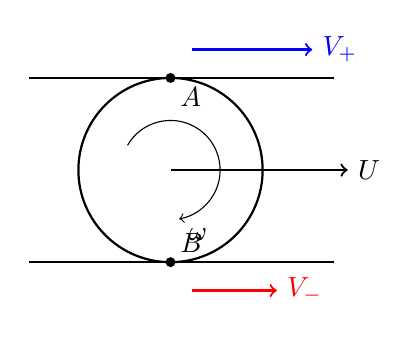
\begin{tikzpicture}[scale=.9]
\draw[thick](-2,1.3)--(2.3,1.3) (-2,-1.3)--(2.3,-1.3);\draw[thick](0,0)circle(1.3);
\fill(0,1.3)circle(2pt)node[below right]{$A$};\fill(0,-1.3)circle(2pt)node[above right]{$B$};
\draw[->,blue,thick](.3,1.7)--(2,1.7)node[right]{$V_+$};\draw[->,red,thick](.3,-1.7)--(1.5,-1.7)node[right]{$V_-$};
\draw[->,thick](0,0)--(2.5,0)node[right]{$U$};\draw[->](150:.7)arc(150:-80:.7)node[below right]{$\omega$};
\end{tikzpicture}}
图\ref{fv:k5:plates}中顺时针转动在 $A$处贡献向右的 $r\omega$，在 $B$处贡献向左的 $r\omega$。这就是两条速度式符号相反的几何原因。相加消去转动，相减消去平动：上下板同速只产生平动，等大反向则圆心静止而自转。若只有一处无滑动，便只有一个方程，不能只用几何约束同时确定 $U,\omega$。


\subsection{绳绕线轴与多接触约束}
线轴外半径控制地面滚动，内半径控制绳在切点处的相对线速度。绳从上侧或下侧离开，转动对沿绳速度的贡献符号不同；若绳与水平线夹角变化，还应保留圆心平动的沿绳投影。速度关系可为常数，也可因几何角改变而变化，不能统一套用一个固定倍数。

圆轮夹在两移动表面之间时，应分别列两个接触点的速度方程，联立求圆心速度和自转速度。对曲面从动机构，接触点通常在改变：法向约束给从动杆运动，切向滑动由两物体的具体运动决定。是否无滑动必须来自题设，不能由“接触”二字推出。
\subsection{线轴出绳角变化为何影响加速度}
若外半径 $R$控制地面滚动，内半径 $r$控制绳速，写 $k=r/R$、$\sigma=+1$表示上侧出绳、$\sigma=-1$表示下侧出绳，则固定方向瞬时关系为 $v=U(\cos\alpha+\sigma k)$。若随运动绳角也改变，先用乘积法则，再对余弦求复合导数：
\[\dot v=\dot U(\cos\alpha+\sigma k)+U(-\sin\alpha)\dot\alpha.\]
移项并在 $\cos\alpha+\sigma k\ne0$时相除，得到
\[\dot U=\frac{\dot v+U\sin\alpha\,\dot\alpha}{\cos\alpha+\sigma k}.
\]
所以恒定拉绳速率并不一般保证圆心匀速，仍需由绳路几何求 $\dot\alpha$。若分母接近零，也应先回到未相除的速度约束判断模型是否允许有限运动。对于系在轴上指定物质点的绳，转动速度未必平行绳，转动贡献应另作投影，不能沿用卷绕切点的 $\pm k$。

\subsection{瞬心法的速度条件与加速度限制}
平面运动的瞬心 $I$是刚体速度场中瞬时速度为零的位置，可能位于刚体外部，也可能随时间移动。若角速度非零，选择两个已知速度且速度方向不平行的点，分别作速度的垂线，其交点便是瞬心。在该瞬间，$\bm v_I=0$使速度公式化为绕 $I$的转动关系，故 $v_P=|\omega|IP$，方向垂直 $IP$。两条垂线若重合，仅用这两个点还不能确定 $I$，应增加另一个已知条件；非零且大小方向相同的各点速度则对应纯平动，常把瞬心称为位于无穷远处。

\fig{k5deep:center}{由两点速度的垂线作瞬心，再用到瞬心的距离比较速度}{\begin{tikzpicture}
\draw[axis](0,0)--(4.5,0);\draw[axis](0,0)--(0,3.1);
\coordinate(A)at(0,2.4);\coordinate(B)at(3.2,0);\coordinate(I)at(3.2,2.4);\coordinate(P)at(1.6,1.2);
\draw[world](A)--(B);\draw[guide](A)--(I)--(B) (I)--(P);
\foreach \n in {A,B,I,P}{\fill(\n)circle(1.3pt);}\node[left]at(A){$A$};\node[below]at(B){$B$};\node[above right]at(I){$I$};\node[left]at(P){$P$};
\draw[flow,blue](A)--++(0,-1.28)node[left]{$v_A$};\draw[flow,blue](B)--++(.96,0)node[above]{$v_B$};\draw[flow,red](P)--++(.48,-.64)node[right]{$\bm v_P$};
\node at(1.6,3.4){$v_A/IA=v_B/IB=v_P/IP=|\omega|$};
\end{tikzpicture}}
图\ref{k5deep:center}取沿互相垂直导轨滑动的杆。$A$ 的速度竖直，故 $IA$ 水平；$B$ 的速度水平，故 $IB$ 竖直。这两条线的交点 $I$ 唯一确定本瞬间的速度场。对杆上的 $P$，速度沿 $IP$ 的垂线，长度按 $IP$ 成比例。下一瞬间重新作图时，$I$ 通常已移到新位置，因此图中的 $I$ 不能当作始终固定的转轴。

加速度不能照搬这一步。以平地纯滚动车轮为例，底部瞬心处的物质点速度为零，但其向上加速度非零；如果把它误当作固定转轴，会算出顶部加速度指向底部且大小错误。正确做法是以圆心等已知物质点为基点，保留基点加速度、角加速度切向项与角速度平方向心项，再把矢量投影到所选坐标。

\subsection{光滑接触的二阶条件与法线转动}
设一点被约束在固定光滑曲线 $F(x,y)=0$上，一阶导数给 $F_xv_x+F_yv_y=0$，说明速度切于曲线。再次求导，必须同时微分 $F_x,F_y$与速度：
\[0=(F_{xx}v_x+F_{xy}v_y)v_x+F_xa_x
 +(F_{yx}v_x+F_{yy}v_y)v_y+F_ya_y.\]
对于二阶连续可微的曲线函数，$F_{xy}=F_{yx}$，合并交叉项即得
\[F_xa_x+F_ya_y+F_{xx}v_x^2+2F_{xy}v_xv_y+F_{yy}v_y^2=0.
\]
后面的速度平方项不能省略。以固定圆 $F=x^2+y^2-R^2$为例，便有 $x a_x+y a_y=-(v_x^2+v_y^2)$，即法向加速度必须指向圆心。若仅对“法向速度为零”作形式替换，误写成法向加速度也为零，就把曲线的弯曲信息全部丢失了。

移动曲面还会增加显含时间的导数项，因此通常应从原始几何方程再求导。光滑接触只禁止法向穿透；允许切向滑动时，物质点速度仍可沿界面不同。无滑动又多加一个切向条件，它们必须来自题设并彼此相容。遇到多个接触，应先检查这些条件能否由同一个刚体运动同时满足，再计算未知速度或加速度。

\subsection{曲线交点的二阶变化}
当圆与移动直线相交，或两个圆彼此移动，交点坐标往往可写成根号函数。对它求导时，每个几何参数都应随时间变化；二阶导数中既有驱动加速度项，也有驱动速度平方项。即使各圆心或直线均匀平动，几何交点仍通常具有非零加速度。

几何交点接近相切位置时，根号分母可能趋零。这不违背圆心速度有限，因为邻近构形的交点位置对参数极为敏感；但到相切后，两交点可能消失，不能继续把根号内负数的公式当作真实运动。作图时应把存在范围和上下分支写清，并检查求导后的方向是否与交点升降一致。

\subsection{从滚动约束到轮缘轨迹}
设轮沿水平地面向右纯滚动，以顺时针累积转角 $q$为参数，初始标记在触地点。无滑动先给圆心横坐标 $x_C=Rq$，再由标记相对圆心的转动得到
\[x=R(q-\sin q),\qquad y=R(1-\cos q).
\]
它表明滚动首先限制圆心的平动与自转，轮缘物质点的对地运动还需做矢量合成。圆心走过一周长，并不表示轮缘标记只走一周长。即使标记某时刻接触地面而速度为零，下一瞬间它也离开接触位置，不能继续把这个物质点当作固定支点。

\fig{k5deep:cycloid}{同一轮缘标记的轨迹为摆线，圆心轨迹为直线}{\begin{tikzpicture}
\begin{scope}[scale=.8]
\draw[world](-.5,0)--(7.4,0);\draw[guide](0,1)--(7,1);
\draw[world,blue]plot[domain=0:360,samples=120]({rad(\x)-sin(\x)},{1-cos(\x)});
\draw[gray,thick](1.570796,1)circle(1);\fill(.570796,1)circle(1.6pt)node[left]{$P$};\fill(1.570796,1)circle(1.3pt)node[right]{$C$};
\draw[guide](1.570796,1)--(.570796,1);\draw[flow,red](.570796,1)--(1.3,1.729204)node[above]{$\bm v_P$};
\foreach \x/\lab in {0/0,3.141593/\pi,6.283185/2\pi}{\node[below]at(\x,0){$q=\lab$};}\node[right]at(6.7,1){圆心};
\end{scope}
\end{tikzpicture}}
图\ref{k5deep:cycloid}在 $q=\pi/2$ 画出轮子，标记位于圆心左侧。其向右平动与相对圆心向上运动合成斜向右上的速度；到 $q=\pi$ 时标记升到顶部，再到 $q=2\pi$ 时重新触地。两个触地尖点的水平距离是 $2\pi R$，这只是圆心前进的距离，标记沿拱形轨迹走过的路程须另行积分。

从圆心向右速度 $U=R\dot q$出发，对两个坐标分别求导：
\[
 \dot x=R(\dot q-\cos q\,\dot q)=U(1-\cos q),\qquad
 \dot y=R\sin q\,\dot q=U\sin q.
\]
先算速率平方，再用半角恒等式，
\[
 v^2=U^2[(1-\cos q)^2+\sin^2q]
 =2U^2(1-\cos q)=4U^2\sin^2\frac q2.
\]
取非负根得到 $v=2|U\sin(q/2)|$，顶部为圆心速率两倍，触地时为零。第六讲将继续求其二阶导数与曲率；此处先检查初相位、滚动正向和三个特殊位置，使后续运算有明确的几何依据。

